% !TEX encoding = UTF-8
% !TEX TS-program = pdflatex
% !TEX root = ../tesi.tex

%**************************************************************
\chapter{Volume Rendering e Qt}
\label{cap:teoria-stage}
%**************************************************************

%**************************************************************
\section{Radiologia e rendering}
\intro{Concetti di base, teoria, algoritmi e gestione/caricamento immagini DICOM}\\

\subsection{Visualizzare informazioni}\label{sec:visualizzare-informazioni}
Visualizzare fa parte della nostra vita quotidiana: dalle mappe satellitari alla computer grafica dell'industria dell'intrattenimento, possiamo trovare esempi di visualizzazione praticamente ovunque. Ma che cosa significa visualizzare informazioni? Informalmente, visualizzare è la trasformazione di dati o informazioni in immagini. Visualizzare coinvolge la vista e la potenza di elaborazione della mente, con un risultato semplice ed efficace per comunicare informazioni complesse e/o voluminose.
\\
Tuttavia, forse la migliore definizione di visualizzazione si trova negli esempi. In molti casi la visualizzazione sta influenzando la vita delle persone e compiendo imprese che alcuni anni fa sarebbero state inimmaginabili, come nella medicina moderna, ambito su cui ci concentreremo.

\subsection{Volumi radiologici}\label{sec:volumi-radiologici}
Le tecniche di diagnostica per immagini, soprattutto in radiologia, sono diventate un importante strumento nella medicina moderna. Ci concentreremo su tecniche come la tomografia computerizzata (TC) e la risonanza magnetica (RM).
\\
Queste teniche utilizzano dei processi di acquisizione e campionamento per raccogliere informazioni sull'anatomia interna di un paziente. Queste informazioni sono raccolte in forma di piani di taglio o in immagini in sezione trasversale di un paziente, in maniera simile a come accade per radiografie a raggi X convenzionali. La TC utilizza un fascio di raggi X per acquisire i dati, mentre la RM utilizza un forte campo magnetico unito a  impulsi a radiofrequenza. Varie teniche matematiche vengono utilizzate per ricostruire i piani di taglio da salvare, dopodichè solitamente, questi vengono raccolte in un volume di dati.
\\
Un'immagine radiologica, o una fetta del volume nel nostro caso, è acquisita come una serie di valori che rappresenta l'attenuazione dei raggi X (nella TC) o il rillassamento dello spin di un atomo. Ogni immagine contiene tutti questi dati in un array, o in una matrice, tuttavia la quantità di dati è così grande che è impossibile comprenderli nella loro forma "grezza". Per questo, assegnandogli una scala di grigi e visualizzandoli su uno schermo, si riesce finalmente a visualizzare la struttura, permettendoci di visualizzare ciò che il computer vede come un insieme di valori come una sezione del corpo umano.

\subsection{Basi di rendering}\label{sec:basi-rendering}
La computer grafica è il processo di generare immagini utilizzando il computer, questo processo viene chiamato rendering. Ci sono molti tipi di rendering, dal disegno 2D a tecniche 3D sofisticate. In questa sezione vedremo le basi del rendering 3D.
\\
Nel mondo reale quando guardiamo un oggetto, per esempio una scatola, i raggi di luce emessi da una sorgente luminosa (per esempio il sole) sono emessi in tutte le direzioni. Alcuni di questi colpiscono la scatola che ne assorbe una parte di luce e ne riflette il resto. Una parte di questa luce riflessa potrebbe dirigersi verso di noi ed entrare nei nostri occhi, se questo succede noi riusciamo a vedere l'oggetto. Allo stesso modo se della luce colpisce il terreno una parte si rifletterà nei nostri occhi.

\begin{figure}[h]
    \centering
    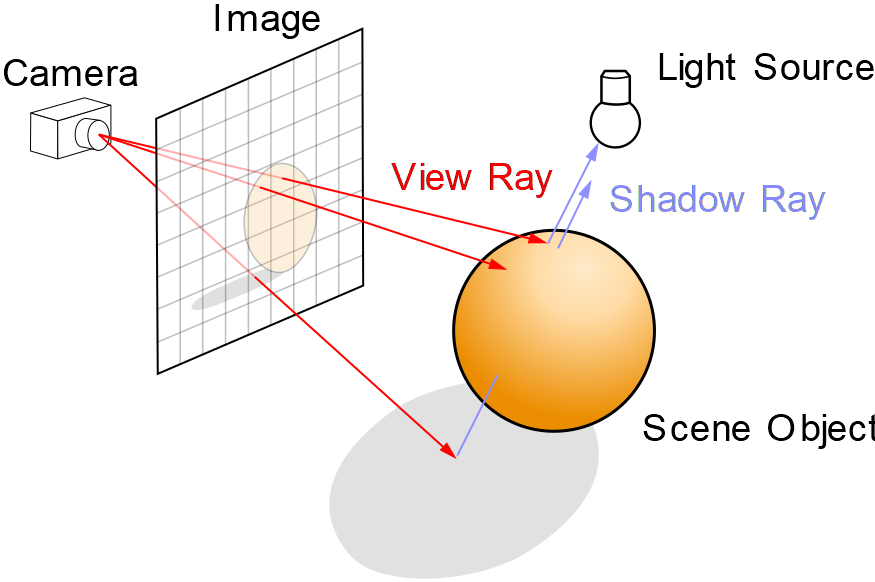
\includegraphics[width=0.5\textwidth]{immagini/ray_tracing_diagram.png}
    \caption{\textit{Algoritmo di Ray-Tracing}}
    \textbf{Fonte}: \href{https://en.wikipedia.org/wiki/Ray_tracing_(graphics)}{wikipedia.org/wiki/Ray\_tracing}
    \label{fig: Algoritmo di Ray-Tracing}
\end{figure}

Una tecnica comune ed efficace per la computer grafica 3D è il ray-tracing, a volte chiamata anche ray-casting. Il ray-tracing simula l'interazione della luce con gli oggetti, seguendo il percorso di ogni raggio. Di solito, si segue il raggio dall'indietro, dalla posizione dell'osservatore (la camera nello schema) nel mondo per determinare che cosa il raggio colpisce. La direzione del raggio quindi, è la direzione che si sta osservando. Quando un raggio colpisce un oggetto, possiamo determinare se quel punto è illuminato da una sorgente di luce: questo viene fatto tracciando un raggio dal punto di intersezione alla luce: se il raggio colpisce qualcos'altro prima di raggiungere la sorgente luminosa, allora quella luce non contribuirà a illuminare il punto. Se ci sono N sorgenti luminose, questo andrà fatto per oguna di esse.
\\
Per chi non avesse mai sentito parlare del ray-tracing, sarà sorprendente scoprire che non è quasi mai usato nella grafica real-time. Questo perchè il ray-tracing è un processo molto lento e dispendioso in termini di risorse, oltre al fatto che fino a pochi anni fa era possibile implementarlo solo via software, per questo sono state sviluppate altre teniche che generano immagini sfruttando meglio l'accellerazione hardware.
\\
La spiegazione fino a questo punto ha assunto che stessimo facendo il render di un oggetto solido. Tuttavia, oggetti come nuvole, l'acqua, la nebbia sono "traslucidi" o diffondono la luce che li attraversa, questi oggetti non possono essere renderizzati utilizzando esclusivamente le interazioni sulle superfici. Dobbiamo invece considerare le proprietà mutevoli all'interno dell'oggetto per mostrarlo correttamente. Ci riferiamo quindi a due modelli di rendering:
\begin{itemize}
\item surface rendering: fare il render della superficie di un oggetto;
\item volume rendering: fare il rendering della superficie e dell'interno di un oggetto.
\end{itemize}

Le tecniche di volume rendering ci consentono di vedere la "disomogeneità" all'interno degli oggetti. Nella TC per esempio, possiamo riprodurre realisticamente immagini a raggi X considerando i valori di intensità sia sulla superficie che all'interno. Vedremo più dettagli sul volume rendering nella prossima sezione, ma tornando all'esempio del ray-tracing, si può immaginare come i raggi non interagiscano solo con la superficie di unh oggetto, ma anche con ciò che è al suo interno.

\section{Volume rendering}
\subsection{Basi di volume rendering}\label{sec:volume-rendering-details}

%**************************************************************
\section{VTK}
\intro{Funzionalità libreria, rendering, taglio, CPU/GPU e funzioni di trasferimento}\\

%**************************************************************
\section{Integrazione con Qt}

%**************************************************************
\section{Software}
\intro{Probabile menzione a Slicer3D, il principale software preso come riferimento}\\

%**************************************************************
\section{Strumenti CTK}

%**************************************************************
\section{Basi di ITK}

